\documentclass[12pt]{article}
\extrafloats{100}
\usepackage{a4wide}
\usepackage{multicol, multirow}
\usepackage[cp1251]{inputenc}
\usepackage[russian]{babel}
\usepackage{amsmath, amsfonts, amssymb, amsthm, amscd}
\usepackage{graphicx, epsfig, subfig, epstopdf}
\usepackage{longtable}
\graphicspath{ {../fig/} }
\begin{document}

\begin{figure}
\centering
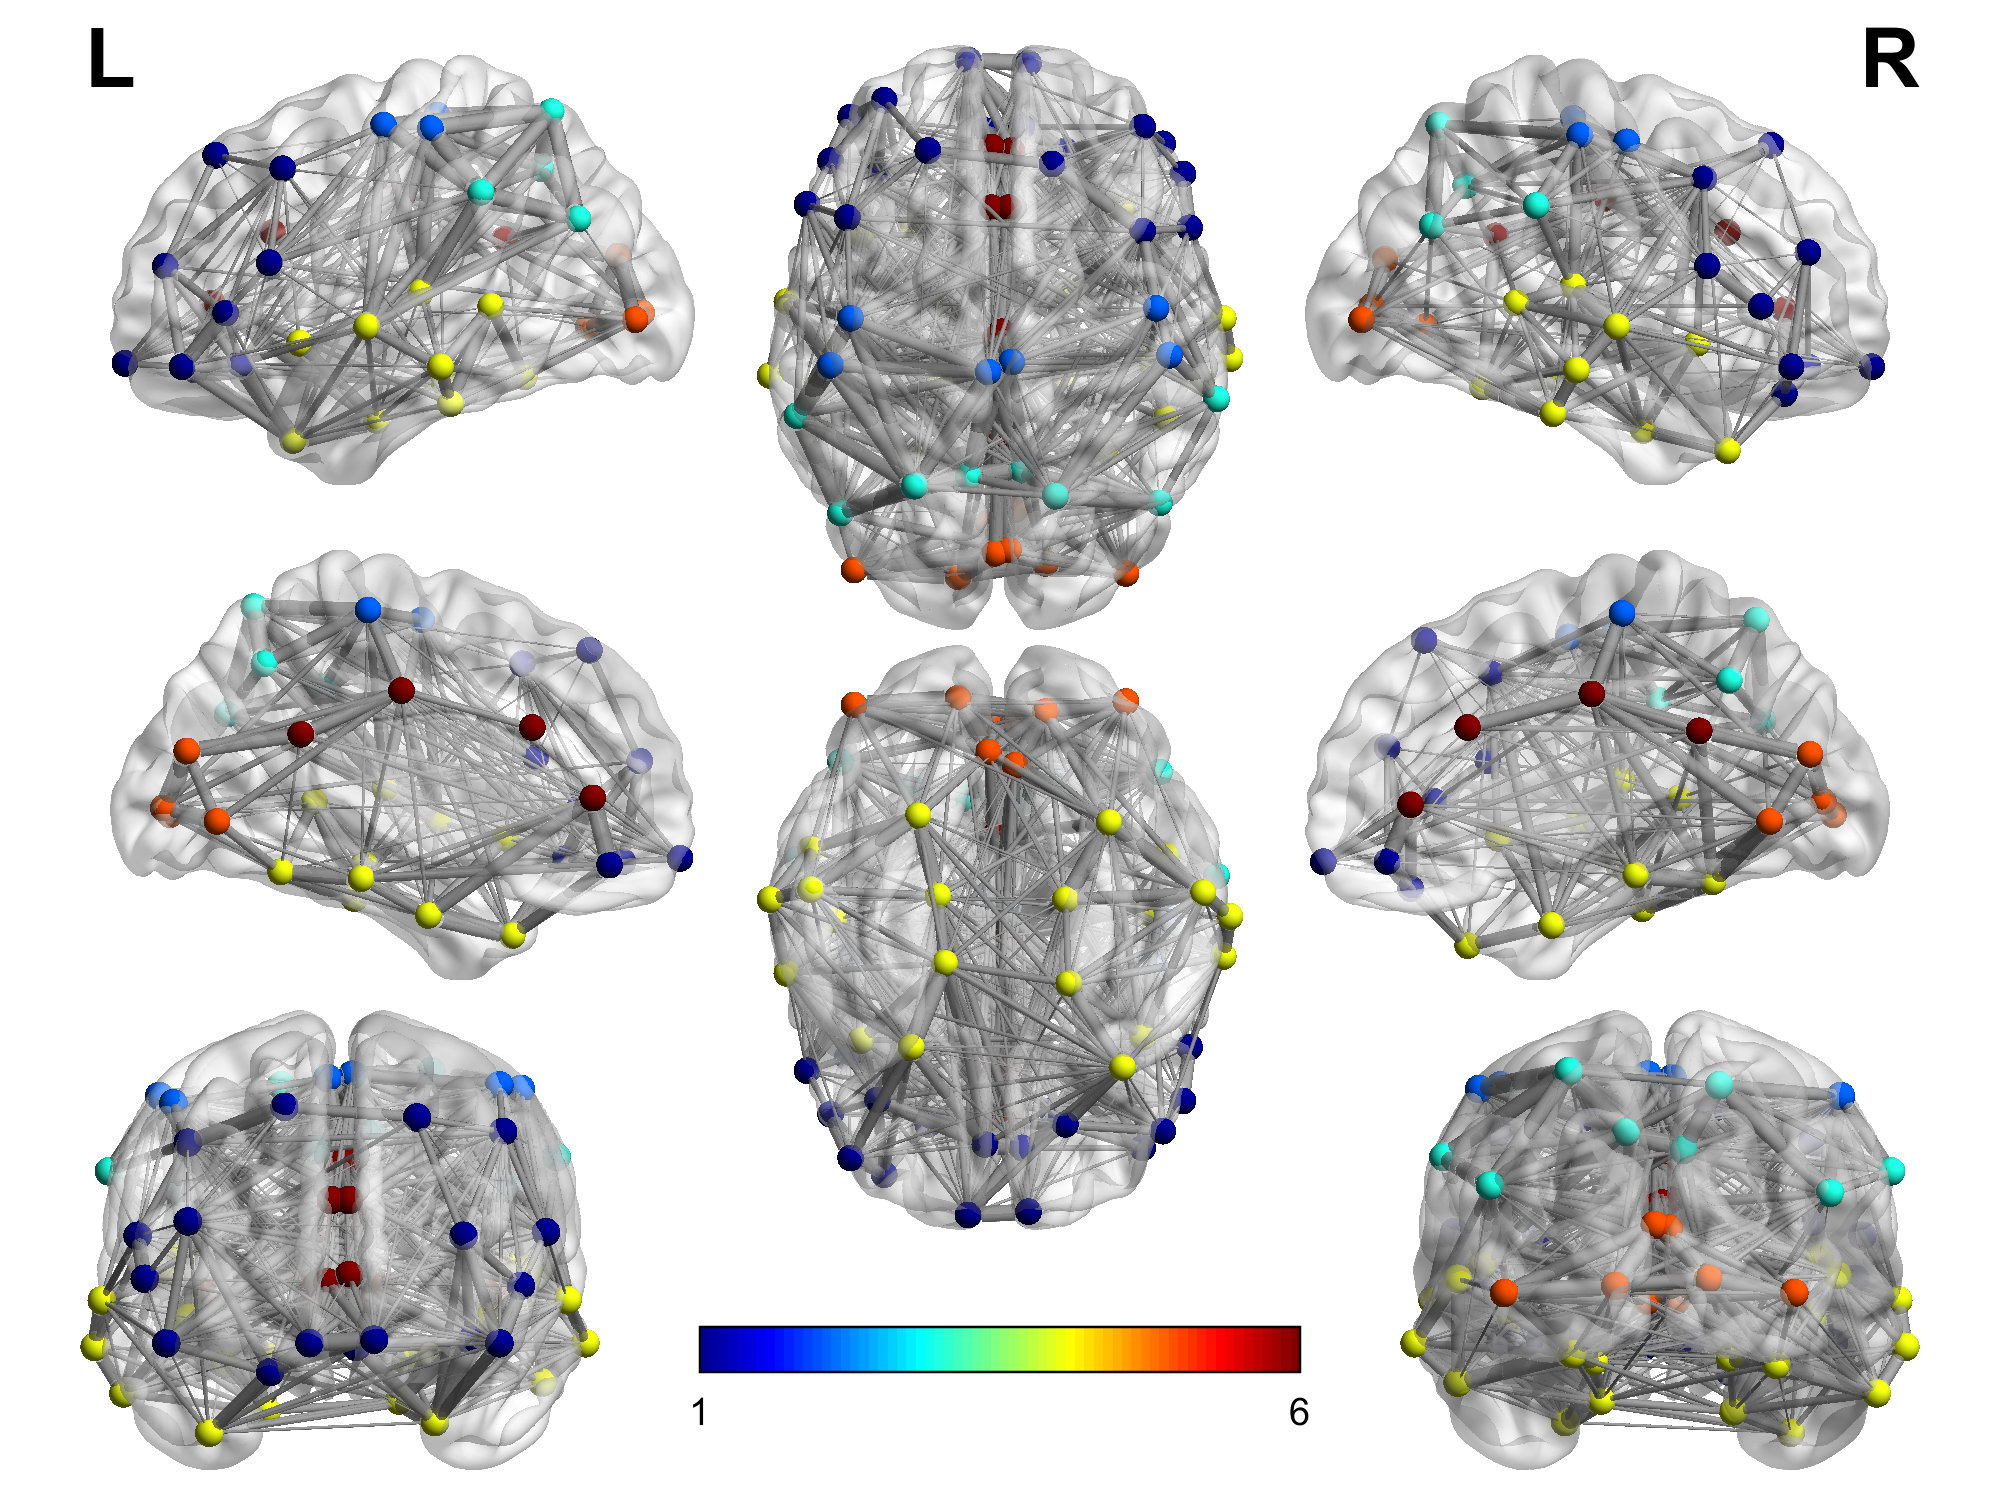
\includegraphics[width=0.8\textwidth]{correlations_early_0p5.png}
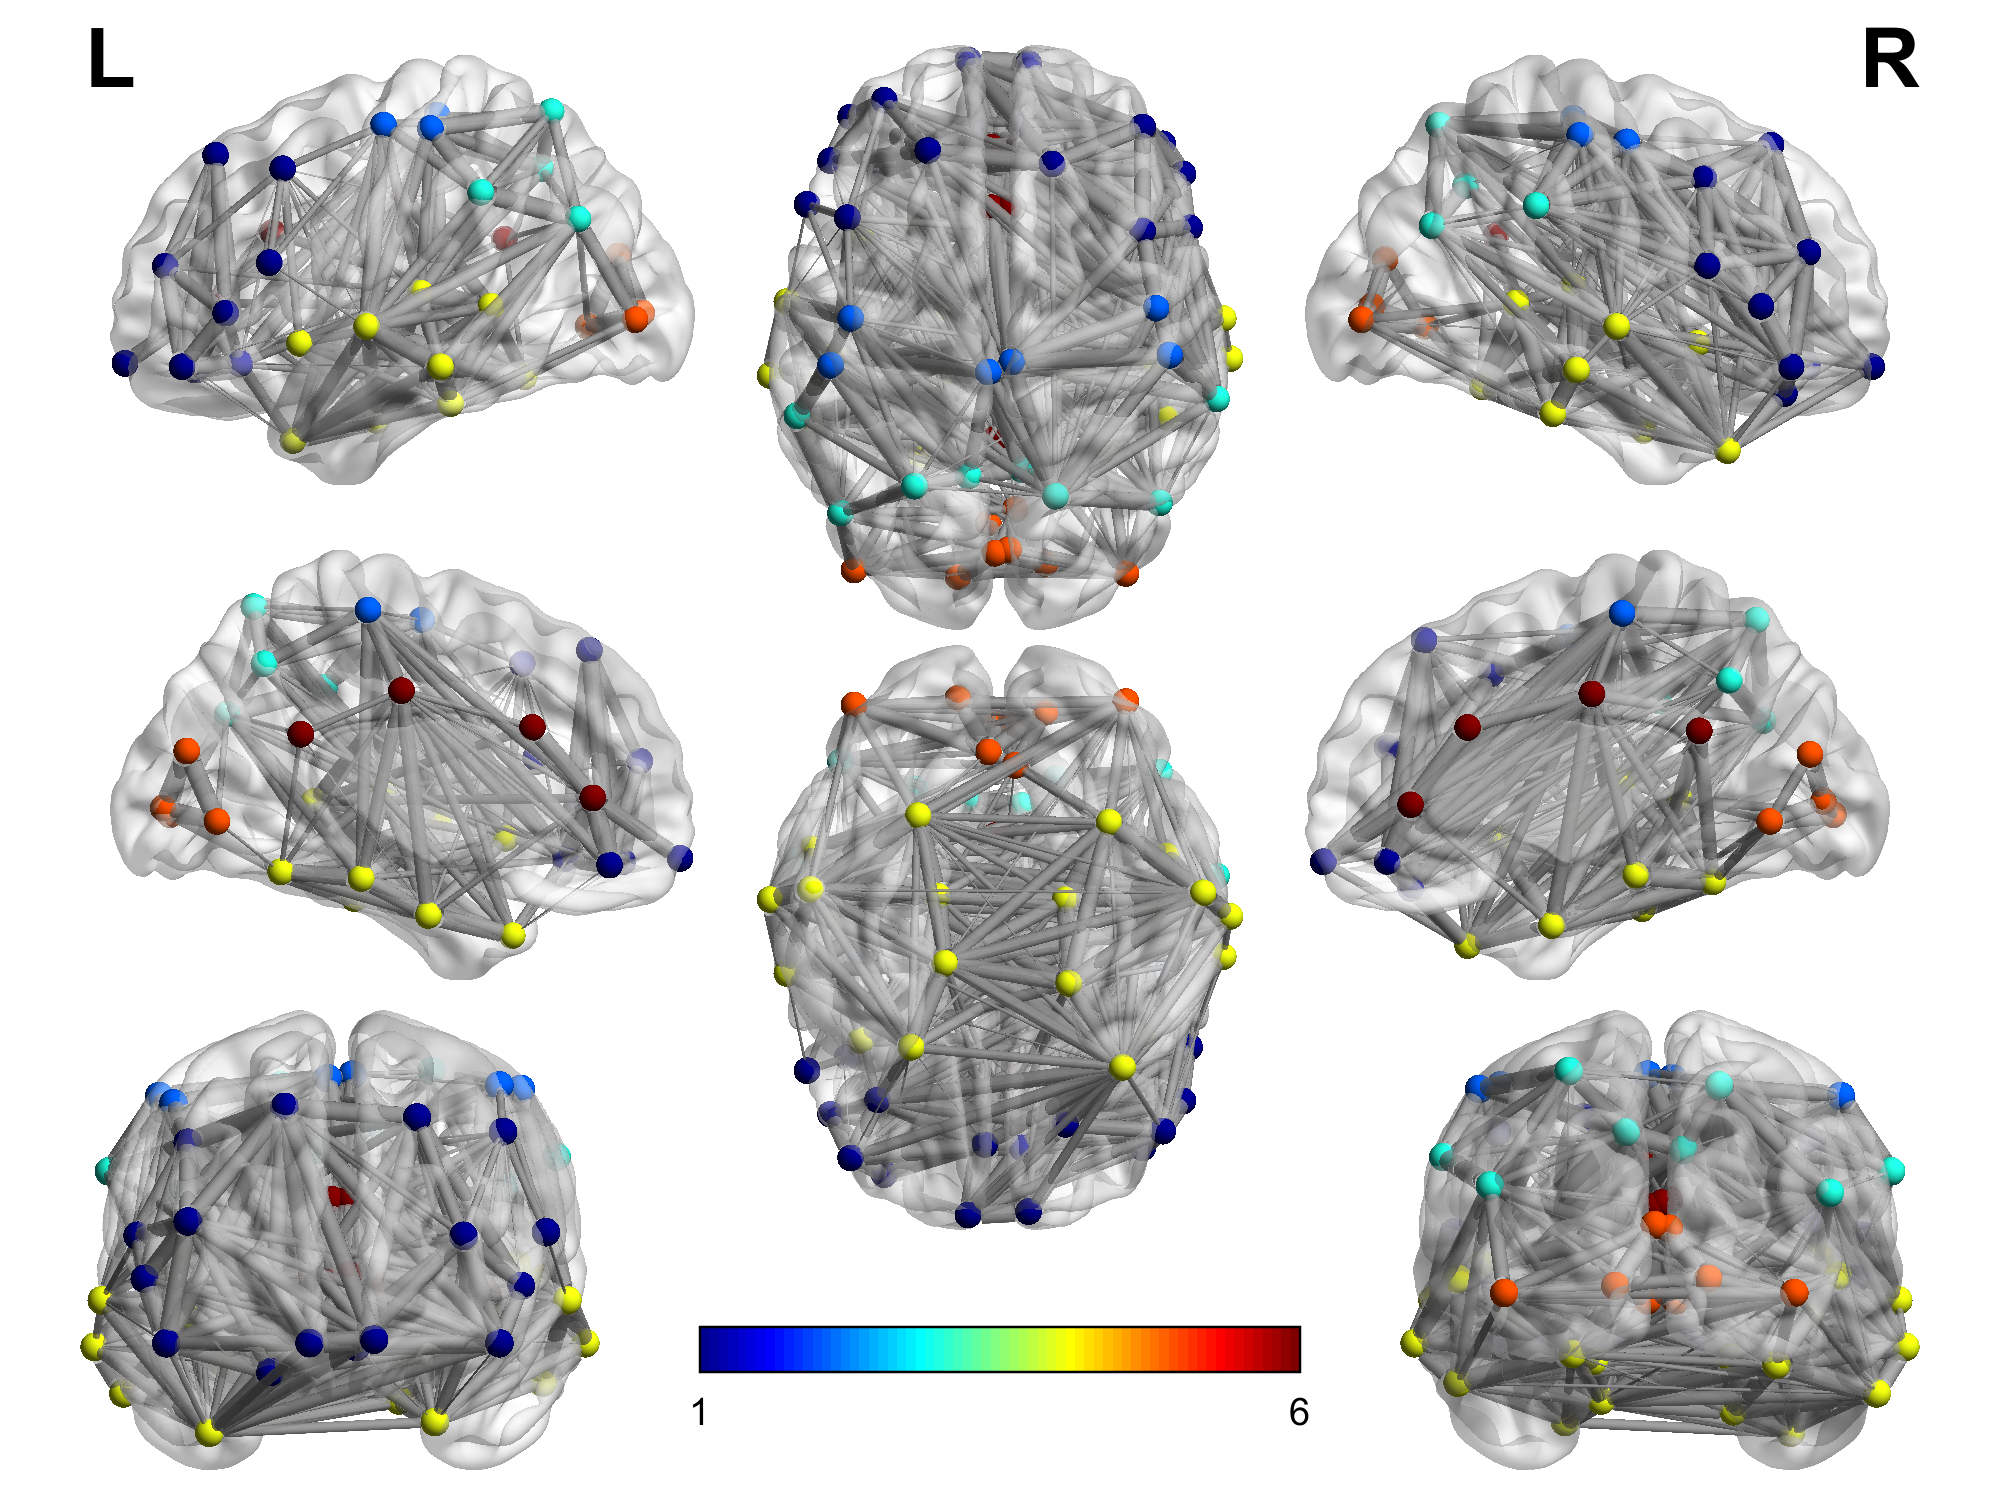
\includegraphics[width=0.8\textwidth]{correlations_late_0p5.png}
\caption{Threshold: 0p5-th quantile.}
\end{figure}


\begin{figure}
\centering
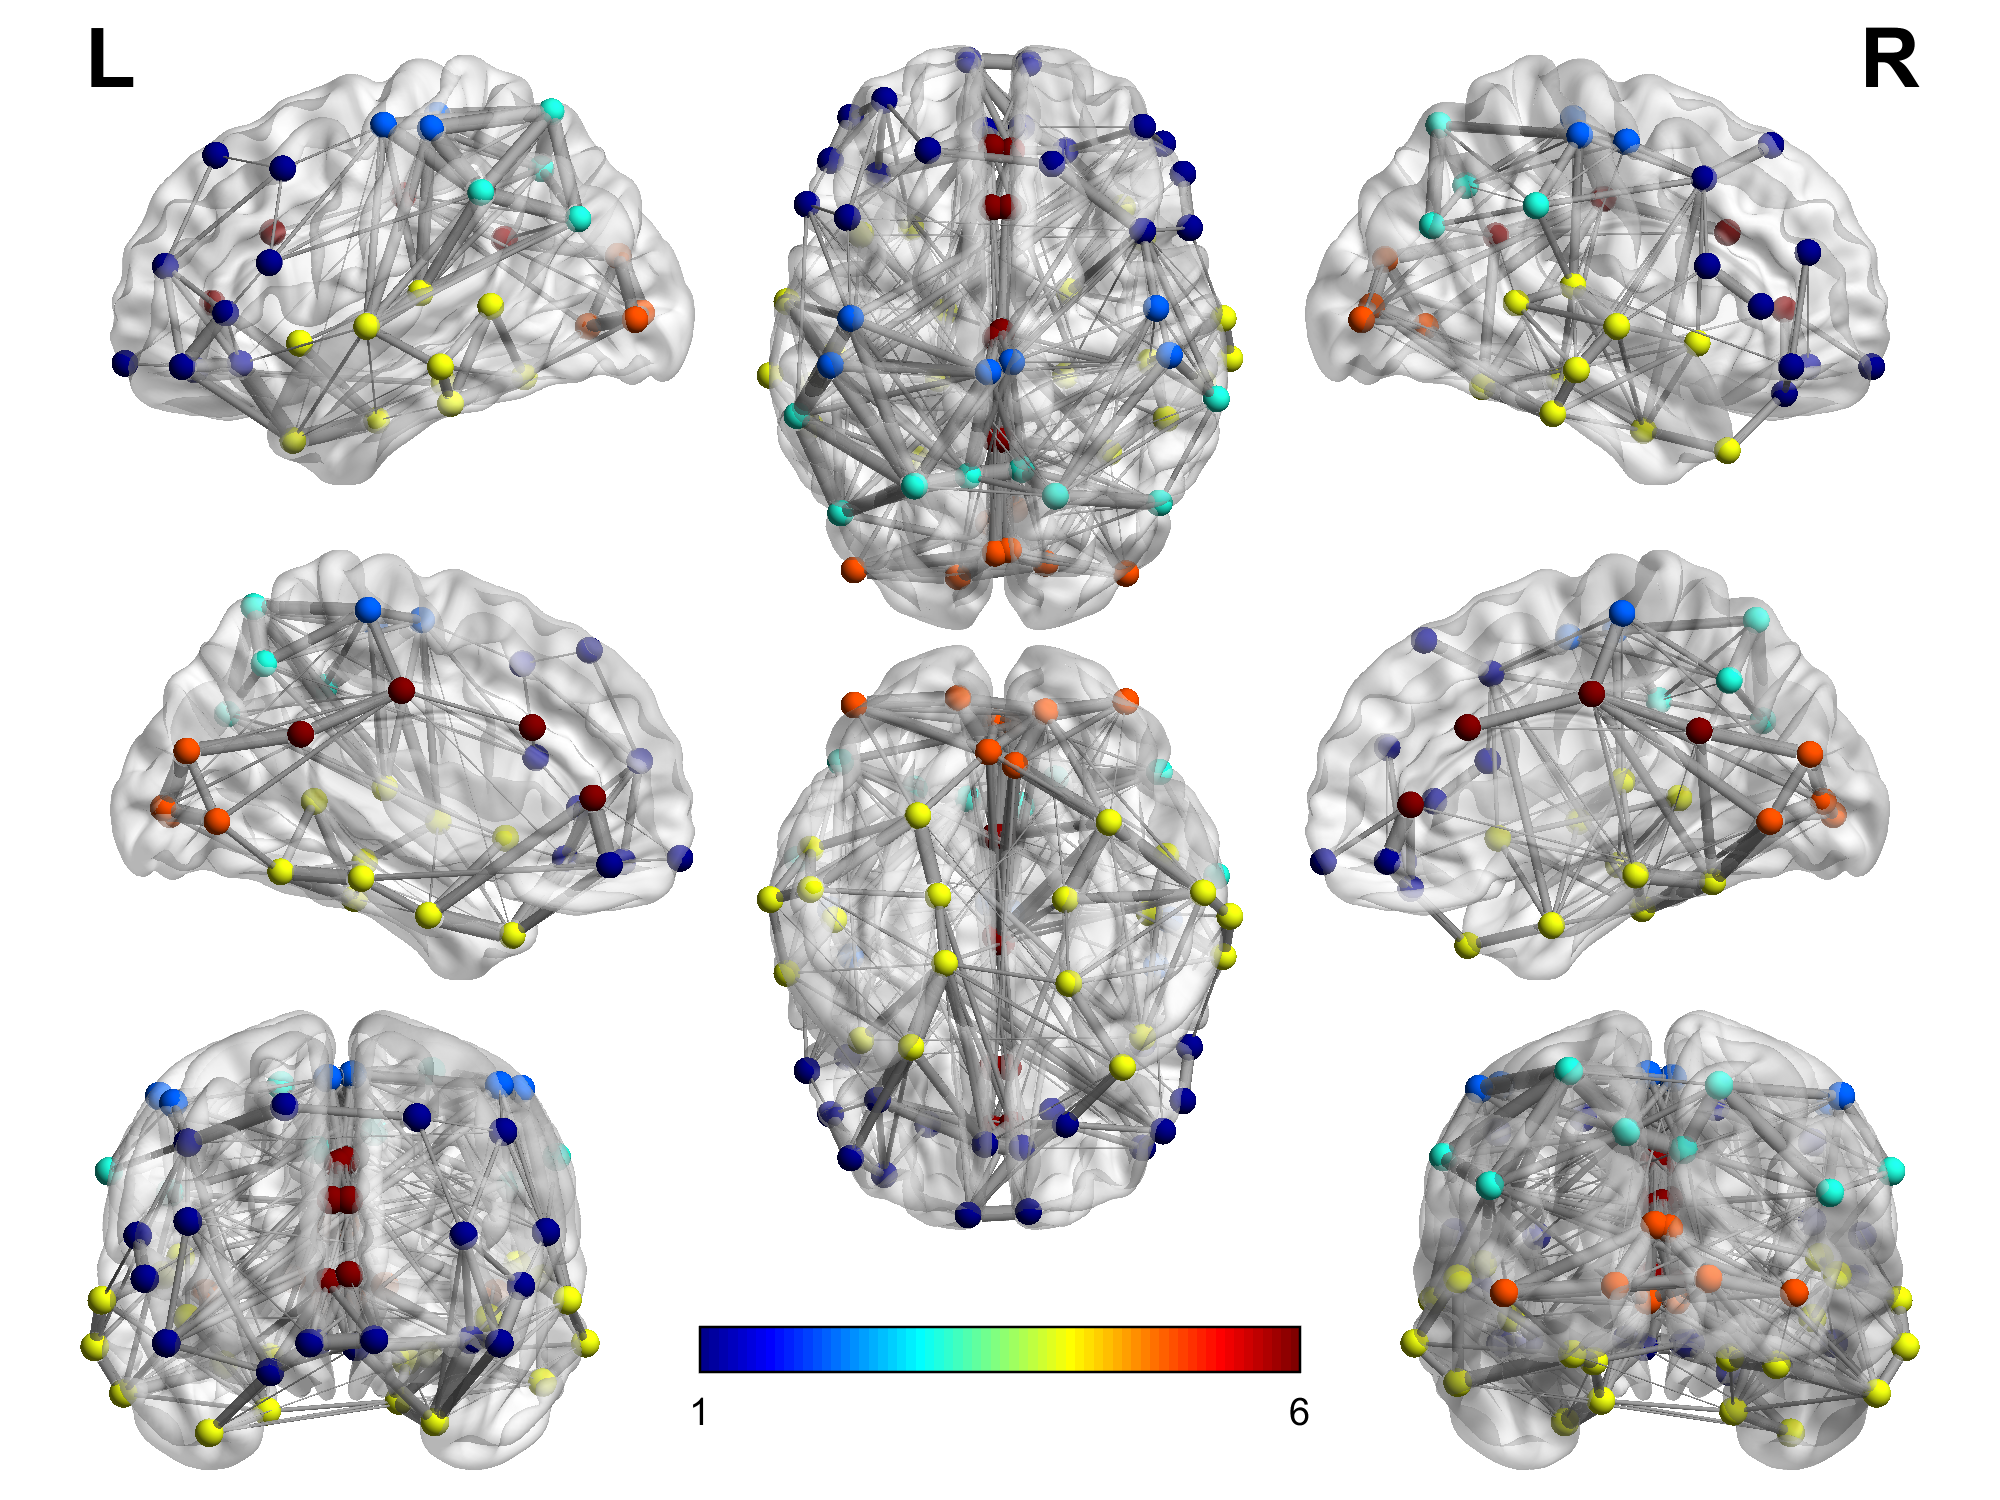
\includegraphics[width=0.8\textwidth]{correlations_early_0p75.png}
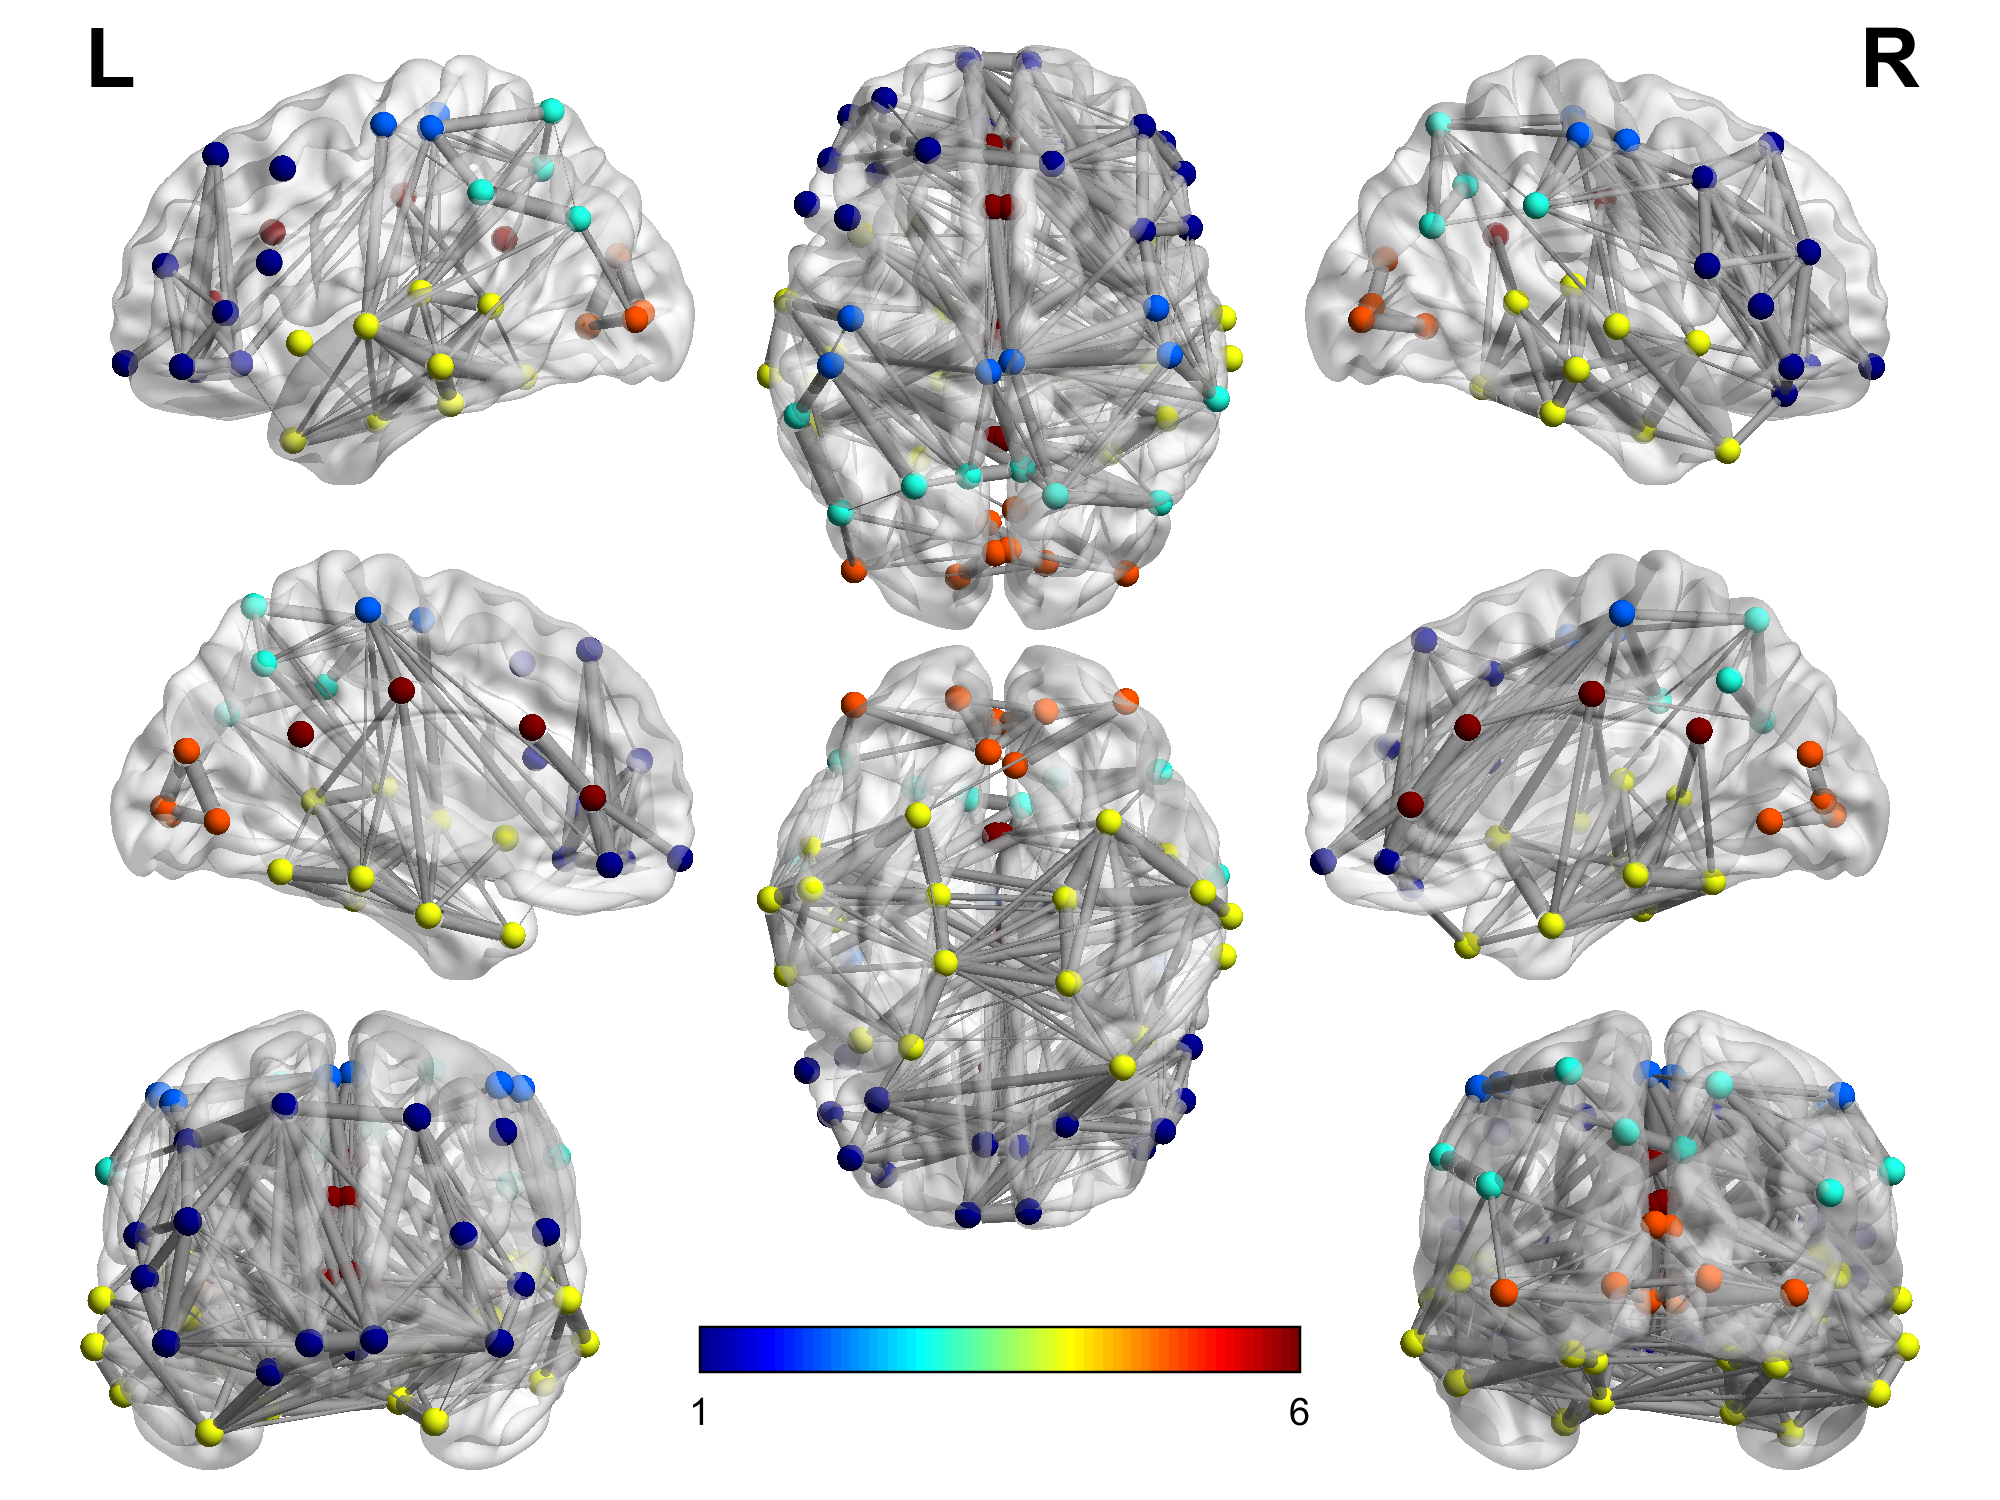
\includegraphics[width=0.8\textwidth]{correlations_late_0p75.png}
\caption{Threshold: 0p75-th quantile.}
\end{figure}


\begin{figure}
\centering
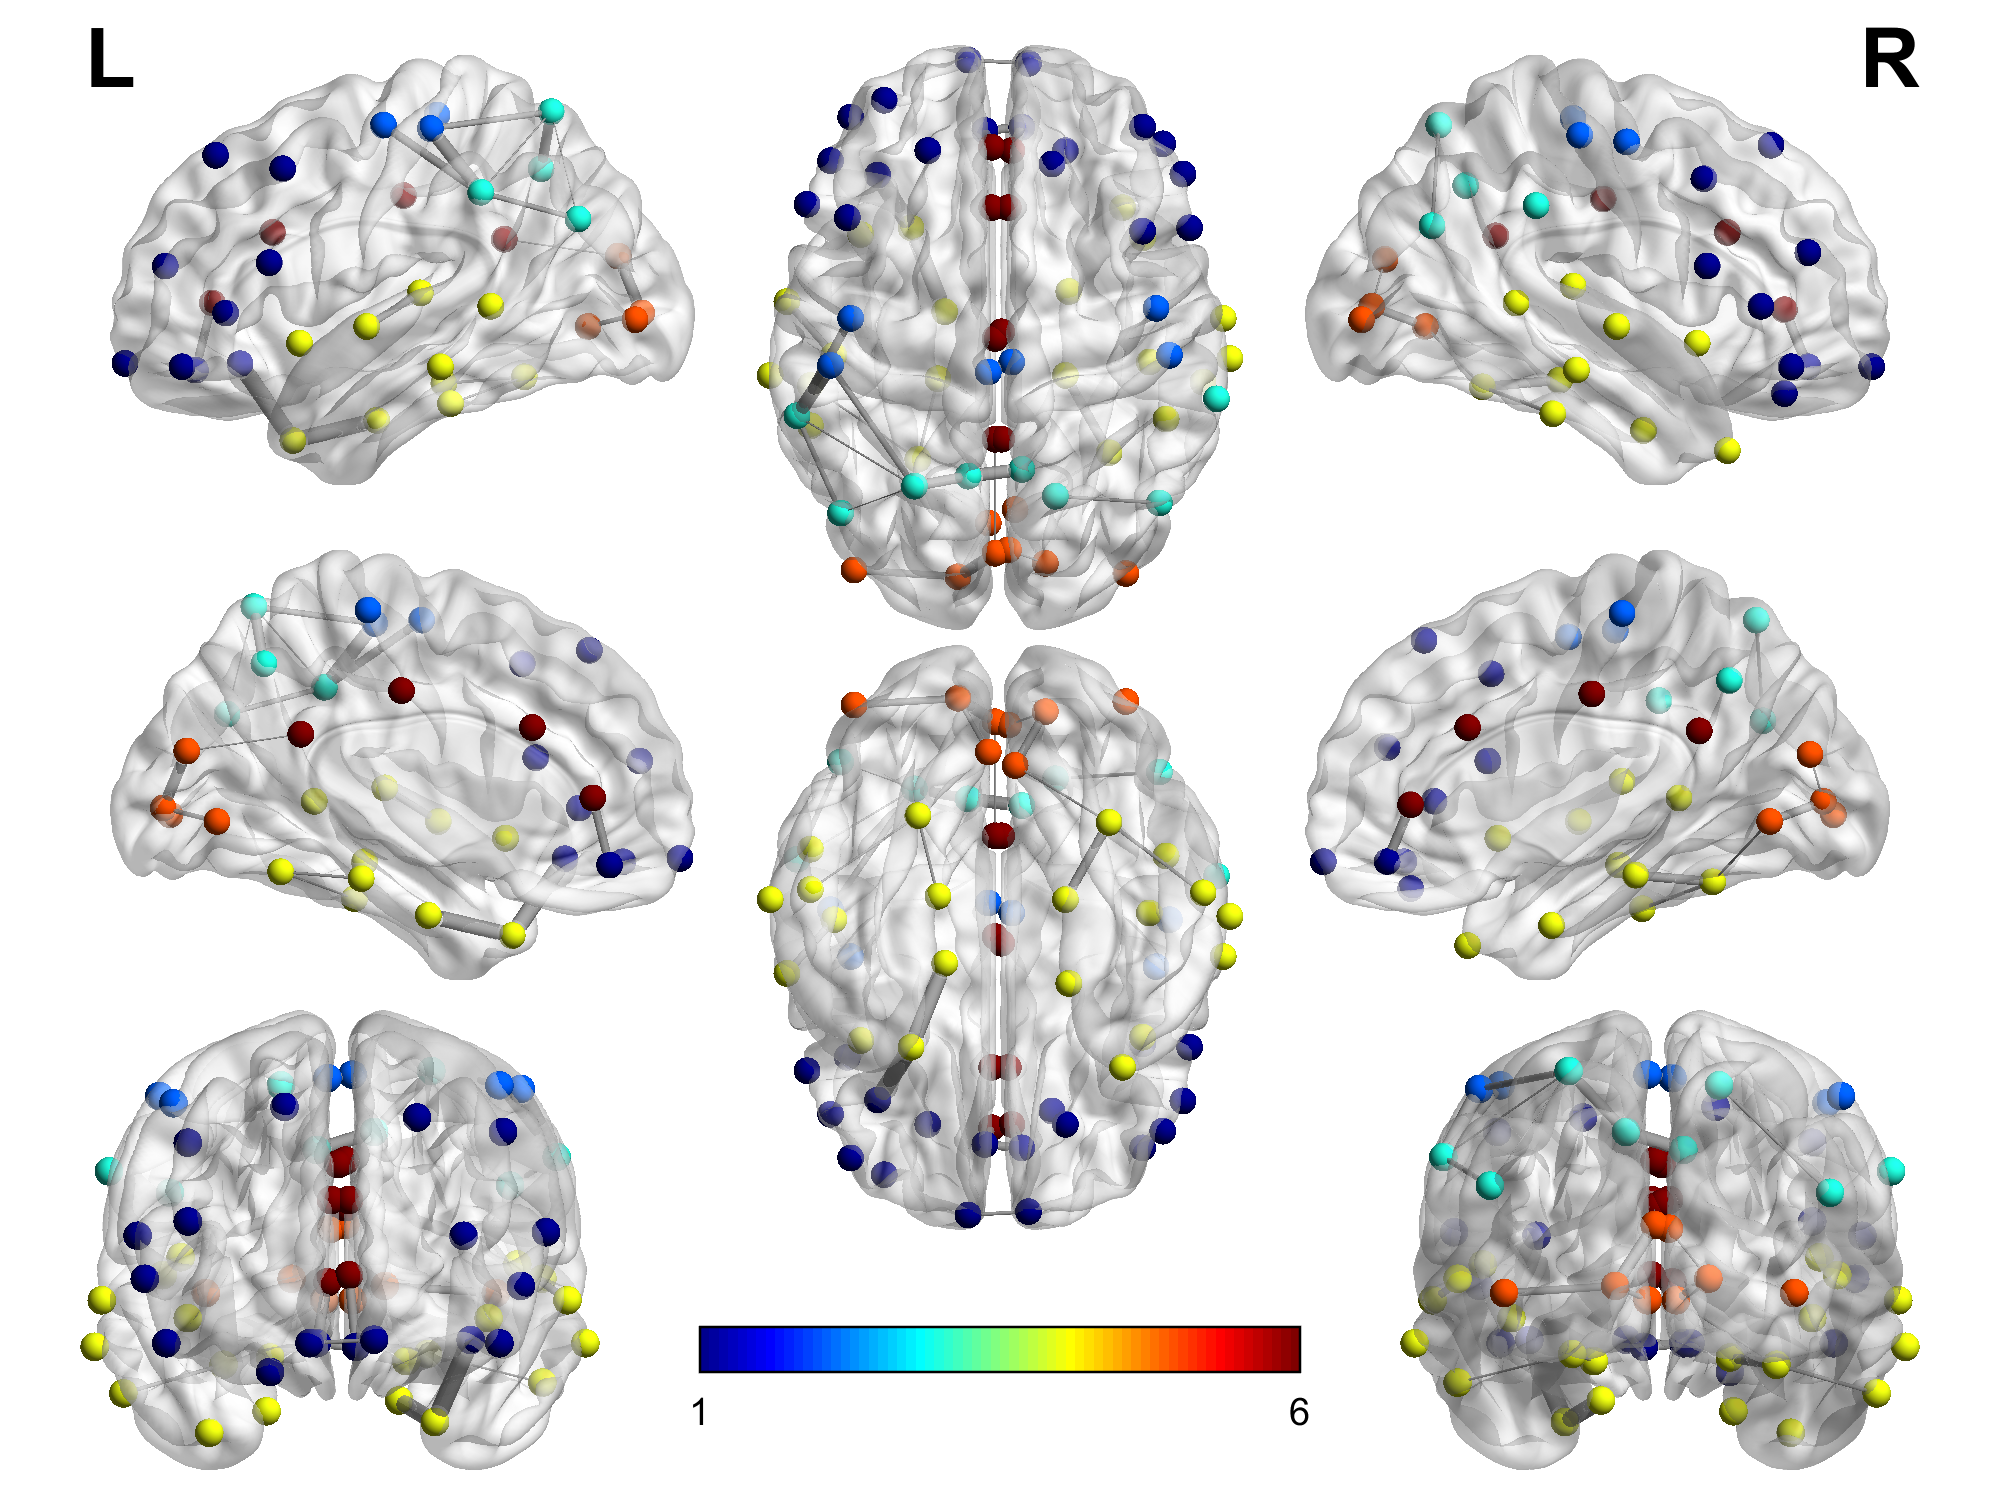
\includegraphics[width=0.8\textwidth]{correlations_early_0p95.png}
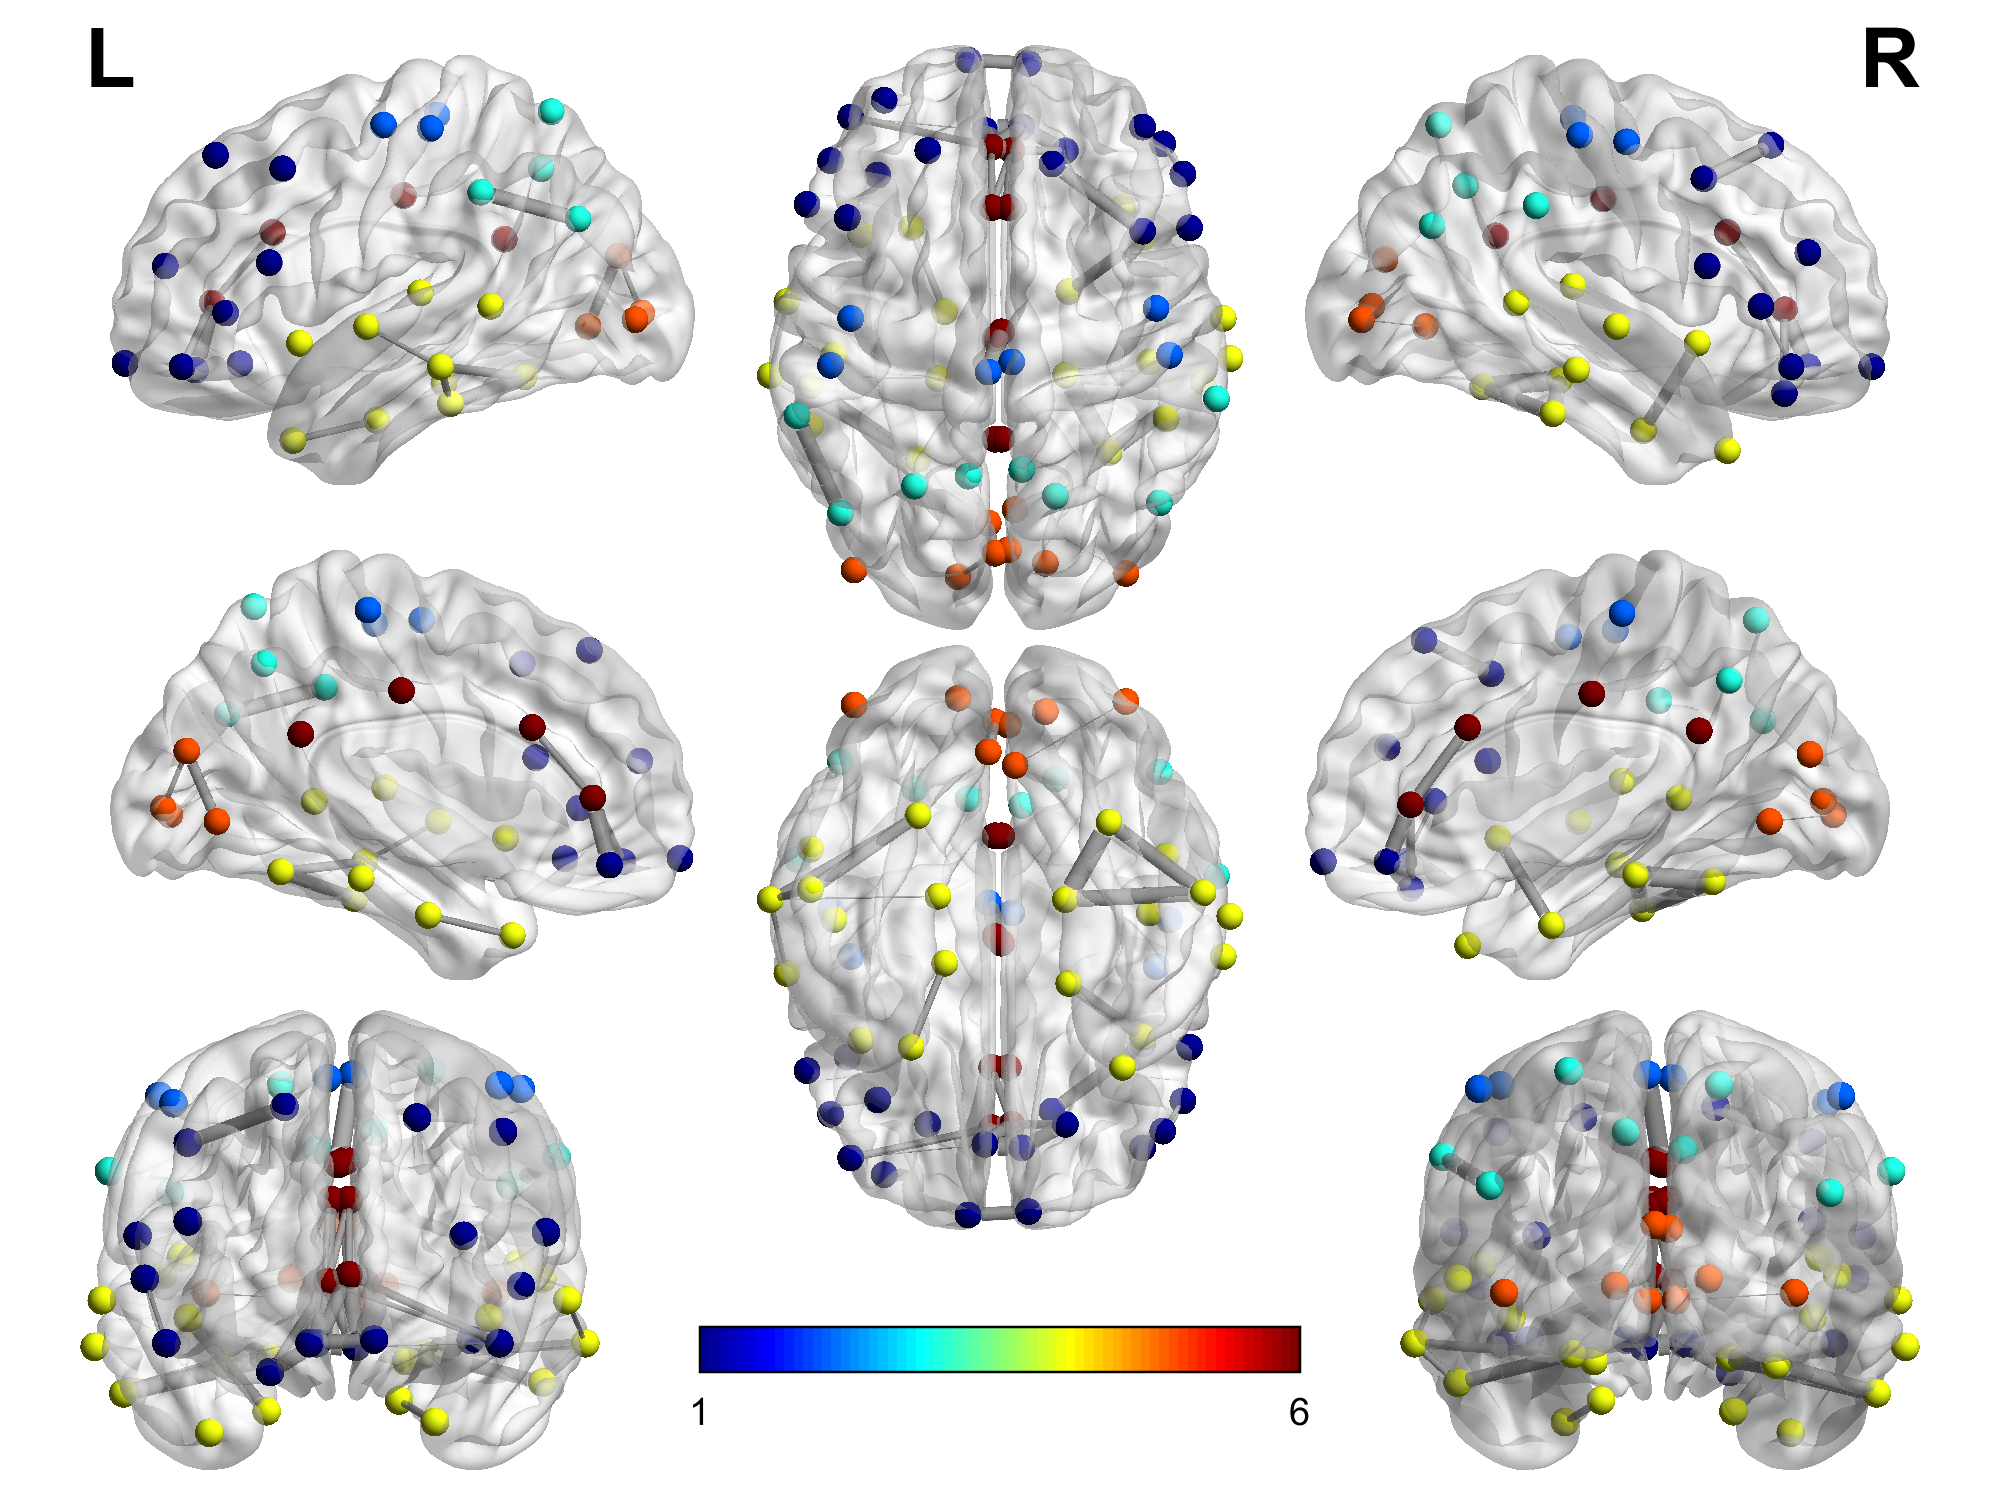
\includegraphics[width=0.8\textwidth]{correlations_late_0p95.png}
\caption{Threshold: 0p95-th quantile.}
\end{figure}


\end{document} 